\section{Dense3d Class Reference}
\label{classDense3d}\index{Dense3d@{Dense3d}}
{\tt \#include $<$dense3d.hpp$>$}

Inheritance diagram for Dense3d::\begin{figure}[H]
\begin{center}
\leavevmode
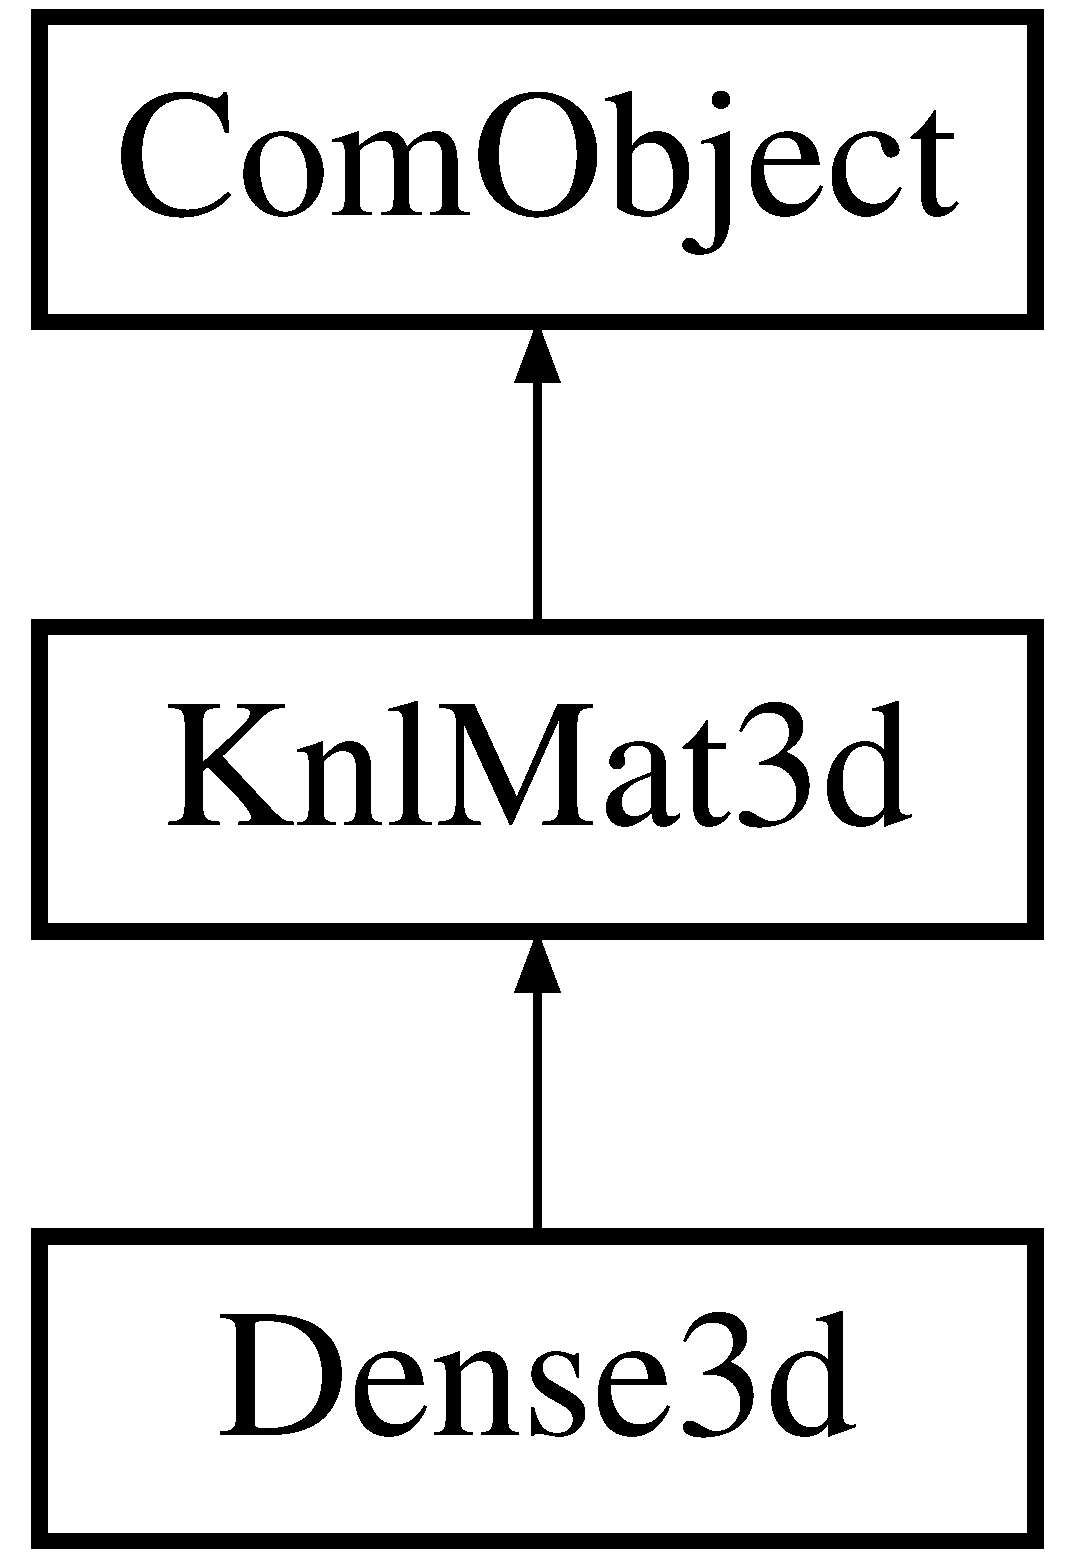
\includegraphics[height=3cm]{classDense3d}
\end{center}
\end{figure}


\subsection{Detailed Description}
Dense3d implements the virtual setup and eval functions of {\bf Knl\-Mat3d}{\rm (p.\,\pageref{classKnlMat3d})} $\ast$/. 



Definition at line 26 of file dense3d.hpp.\subsection*{Public Member Functions}
\begin{CompactItemize}
\item 
{\bf Dense3d} (const string \&p)
\item 
{\bf $\sim$Dense3d} ()
\item 
int {\bf setup} (map$<$ string, string $>$ \&)
\item 
int {\bf evaluate} (const Dbl\-Num\-Vec \&src\-Den, Dbl\-Num\-Vec \&trg\-Val)
\end{CompactItemize}


\subsection{Constructor \& Destructor Documentation}
\index{Dense3d@{Dense3d}!Dense3d@{Dense3d}}
\index{Dense3d@{Dense3d}!Dense3d@{Dense3d}}
\subsubsection{\setlength{\rightskip}{0pt plus 5cm}Dense3d::Dense3d (const string \& {\em p})}\label{classDense3d_26942f58b7764c78dc6281f8bf79c4b5_26942f58b7764c78dc6281f8bf79c4b5}


Dense3d constructor takes string to declare type 

Definition at line 22 of file dense3d.cpp.

\footnotesize\begin{verbatim}22                                : KnlMat3d(p)
23 {
24 }
\end{verbatim}\normalsize 


\index{Dense3d@{Dense3d}!~Dense3d@{$\sim$Dense3d}}
\index{~Dense3d@{$\sim$Dense3d}!Dense3d@{Dense3d}}
\subsubsection{\setlength{\rightskip}{0pt plus 5cm}Dense3d::$\sim$Dense3d ()}\label{classDense3d_465b01ffd81006def662ecab05e22099_465b01ffd81006def662ecab05e22099}


Dense3d destructor 

Definition at line 26 of file dense3d.cpp.

\footnotesize\begin{verbatim}27 {
28 }
\end{verbatim}\normalsize 




\subsection{Member Function Documentation}
\index{Dense3d@{Dense3d}!evaluate@{evaluate}}
\index{evaluate@{evaluate}!Dense3d@{Dense3d}}
\subsubsection{\setlength{\rightskip}{0pt plus 5cm}int Dense3d::evaluate (const Dbl\-Num\-Vec \& {\em src\-Den}, Dbl\-Num\-Vec \& {\em trg\-Val})\hspace{0.3cm}{\tt  [virtual]}}\label{classDense3d_3d2ce8cfb3d9632d6b69352f1bb5eda2_3d2ce8cfb3d9632d6b69352f1bb5eda2}


Virtual evaluation function 

Implements {\bf Knl\-Mat3d} {\rm (p.\,\pageref{classKnlMat3d_fcf3de1e6ce4ee024ef0d320363bd920_fcf3de1e6ce4ee024ef0d320363bd920})}.

Definition at line 39 of file dense3d.cpp.

References Knl\-Mat3d::\_\-knl, Knl\-Mat3d::\_\-src\-Nor, Knl\-Mat3d::\_\-src\-Pos, Knl\-Mat3d::dim(), Kernel3d::kernel(), Knl\-Mat3d::src\-DOF(), and Knl\-Mat3d::trg\-DOF().

\footnotesize\begin{verbatim}40 {
41   //-----------------------------------
42   iA(srcDen.m()==srcDOF()*(*_srcPos).n());  iA(trgVal.m()==trgDOF()*(*_trgPos).n());
43   
44   int dim  = this->dim();
45   int srcDOF = this->srcDOF();
46   int trgDOF = this->trgDOF();
47   /* Number of sources */
48   int numSrc = (*_srcPos).n();
49   /* Number of targets */
50   int numTrg = (*_trgPos).n();
51   
52   DblNumMat inter(trgDOF, numSrc*srcDOF);
53   for(int i=0; i<numTrg; i++) {
54          DblNumMat onePosMat(dim, 1, false, (*_trgPos).clmdata(i));
55          DblNumVec oneValVec(trgDOF, false, trgVal.data()+trgDOF*i);
56          iC( _knl.kernel((*_srcPos), (*_srcNor), onePosMat, inter) );
57          iC( dgemv(1.0, inter, srcDen, 0.0, oneValVec) );
58   }
59   
60   return 0;
61 }
\end{verbatim}\normalsize 


\index{Dense3d@{Dense3d}!setup@{setup}}
\index{setup@{setup}!Dense3d@{Dense3d}}
\subsubsection{\setlength{\rightskip}{0pt plus 5cm}int Dense3d::setup (map$<$ string, string $>$ \&)\hspace{0.3cm}{\tt  [virtual]}}\label{classDense3d_6c9d66eef2ad01ccfea65cb116bf5726_6c9d66eef2ad01ccfea65cb116bf5726}


Virtual setup function 

Implements {\bf Knl\-Mat3d} {\rm (p.\,\pageref{classKnlMat3d_24cbbecf677cd909a522d252feebf2c6_24cbbecf677cd909a522d252feebf2c6})}.

Definition at line 31 of file dense3d.cpp.

References Knl\-Mat3d::\_\-src\-Nor, Knl\-Mat3d::\_\-src\-Pos, Knl\-Mat3d::\_\-trg\-Pos, and Knl\-Mat3d::dim().

\footnotesize\begin{verbatim}32 {
33   iA(_srcPos!=NULL && _srcNor!=NULL && _trgPos!=NULL);
34   iA((*_srcPos).m()==dim() && (*_trgPos).m()==dim());  //nothing to do
35   return 0;
36 }
\end{verbatim}\normalsize 




The documentation for this class was generated from the following files:\begin{CompactItemize}
\item 
fmm3d/{\bf dense3d.hpp}\item 
fmm3d/{\bf dense3d.cpp}\end{CompactItemize}
